\documentclass[a4paper,11pt]{article}
\input{/home/tof/Documents/Cozy/latex-include/preambule_lua.tex}
\newcommand{\showprof}{show them}  % comment this line if you don't want to see todo environment
\fancyhead[L]{TP Construction d'un réseau}
\newdate{madate}{10}{09}{2020}
\fancyhead[R]{Seconde - SNT} %\today
\fancyfoot[L]{~\\Christophe Viroulaud}
\fancyfoot[C]{\textbf{Page \thepage}}
\fancyfoot[R]{\includegraphics[width=2cm,align=t]{/home/tof/Documents/Cozy/latex-include/cc.png}}

\begin{document}
\begin{Form}
\begin{commentprof}
Mettre TP-reseau-fichiers.zip sur site avant cours
\end{commentprof}
\paragraph{Objectif:}Simuler le réseau internet.
\section{Découverte du logiciel Filius}
\subsection{Présentation}
Le logiciel \emph{filius} permet de simuler des réseaux et d'étudier la transmission de données entre machines.
\begin{figure}[!h]
\centering
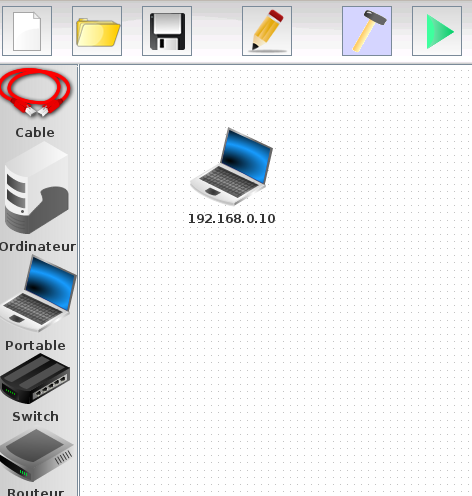
\includegraphics[width=5cm]{ressources/filius-ecran.png}
\captionof{figure}{Présentation de filius}
\label{filius}
\end{figure}
L'écran est séparé en plusieurs parties:
\begin{itemize}
\item le bandeau de gauche propose les différents appareils utilisables dans le réseau. Il faut glisser-déposer la machine sur la scène centrale.
\item Le bandeau haut:
\begin{itemize}
\item Le marteau permet de passer en mode \emph{conception}.
\item La flèche verte permet de passer en mode \emph{simulation}.
\end{itemize}
\item Le bandeau bas (figure \ref{config}) permet de configurer l'appareil sélectionné.
\end{itemize}
\begin{figure}[!h]
\centering
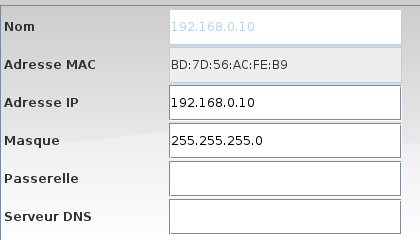
\includegraphics[width=5cm]{ressources/config-pc.png}
\captionof{figure}{Configurer une machine}
\label{config}
\end{figure}
\subsection{Première utilisation}
\begin{activite}
\begin{enumerate}
\item Glisser un portable sur la scène.
\item Le sélectionner et cocher la case en bas à droite \emph{Utiliser l'adresse IP comme nom}. Il faudra effectuer cette opération pour chaque machine.
\item Glisser un second portable.
\item Le sélectionner et modifier son adresse IP en \emph{192.168.0.11}.
\item Relier les deux portables par un câble.
\item Passer alors en mode \textbf{simulation}.
\item Sélectionner une machine. L'écran (figure \ref{machine}) apparaît.
\item Cliquer sur \emph{Installation} et installer l'application \emph{ligne de commande}.
\item Ouvrir \emph{ligne de commande}.
\item Entrer la commande: \textbf{ipconfig}. Vérifier l'adresse de la machine.
\item Entrer la commande: \textbf{ping 192.168.0.11}. Vérifier la connexion avec l'autre portable.
\end{enumerate}
\end{activite}
\begin{figure}[!h]
\centering
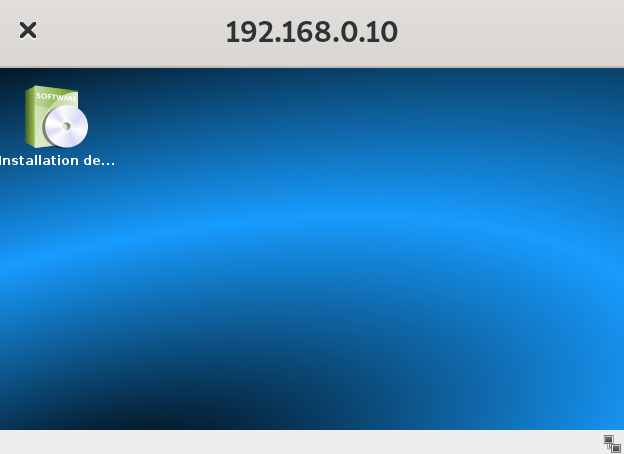
\includegraphics[width=3cm]{ressources/ecran-machine.png}
\captionof{figure}{Installer une application}
\label{machine}
\end{figure}
\section{Repérer une machine}
\begin{figure}[!h]
\centering
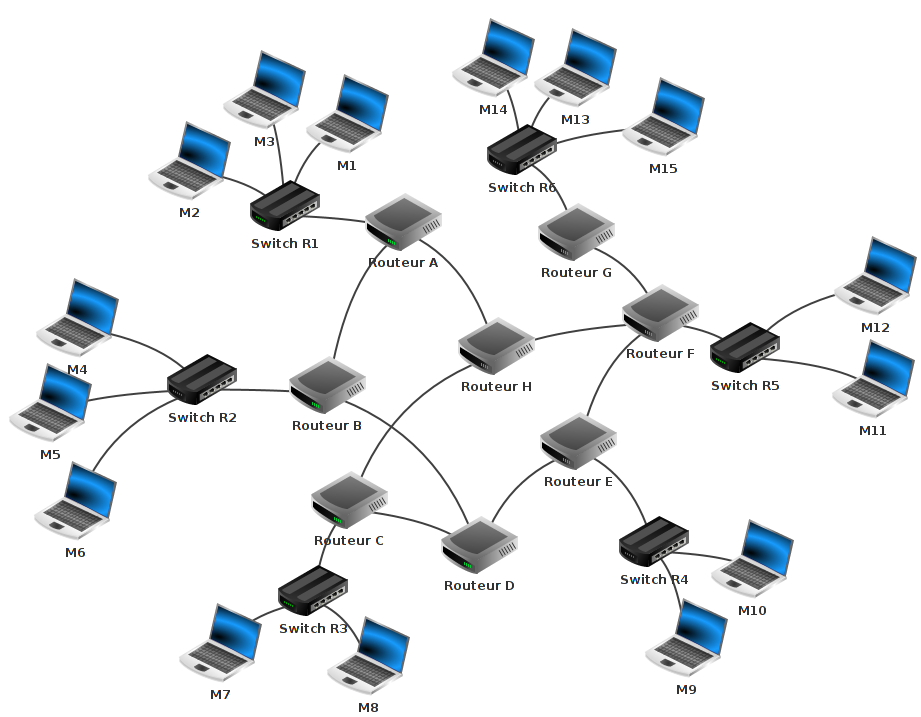
\includegraphics[width=5cm]{ressources/routage.png}
\captionof{figure}{Réseau internet}
\label{reseau}
\end{figure}
\begin{activite}
\begin{enumerate}
\item Depuis le site \url{https://cviroulaud.github.io}, télécharger le dossier compressé \emph{TP réseau fichiers}.
\item Décompresser le dossier dans le dossier \emph{perso} de l'ordinateur. Le fichier \emph{reperer-machine.fls} sera utilisé dans cette activité et l'autre dans le chapitre suivant.
\item Sur la figure \ref{reseau} entourer la partie qui représente le réseau internet.
\item Ouvrir le fichier \emph{reperer-machine.fls} avec le logiciel \emph{filius} et lancer le mode \textbf{simulation}.
\item Repérer les adresses IP des machines M14 et M9.
\item Depuis la console de la machine M14, exécuter la commande \textbf{traceroute adresse\_M9}. Cette commande suit le chemin d'un paquet de données, d'une machine à l'autre.
\item Noter le chemin parcouru.
\item Revenir en mode \textbf{conception} et supprimer le câble entre les routeurs E et F: nous simulons une panne réseau.
\item refaire un \emph{traceroute} entre M14 et M9. Il faudra peut-être attendre quelques secondes afin que les tables de routage se mettent à jour.
\item Noter le nouveau chemin parcouru.
\item Citer la topologie du réseau internet. Donner l'avantage de cette topologie mis en avant dans cette simulation.
\end{enumerate}
\end{activite}
\section{Transmettre des données}
\subsection{Mise en pratique du protocole}
\begin{activite}
\begin{enumerate}
\item Ouvrir le fichier \emph{transmission.fls} et lancer le mode \textbf{simulation}.
\end{enumerate}
La machine \emph{serveur web} est un ordinateur branché sur le réseau internet qui héberge un ou plusieurs sites web. Un ordinateur personnel qui veut afficher un site web utilise un navigateur pour se connecter au \emph{serveur web}.
\begin{enumerate}[resume]
\item Citer au moins deux navigateurs web.
\item Choisir une machine et installer le \emph{navigateur web}.
\item Faire un clic-droit sur la machine et choisir \emph{afficher les échanges de données}. Une fenêtre apparaît.
\item Depuis le navigateur web de la machine accéder à l'adresse \url{http://ip\_serveur\_web}. Quel est le site affiché?
\item Observer la fenêtre \emph{échanges de données}. Quel protocole a été utilisé pour échanger les données entre le portable et le serveur?
\item Combien d'échanges (pour ce protocole) y-a-t-il eu pour afficher la page web?
\end{enumerate}
\begin{commentprof}
quel est le protocole utilisé pour un ping? ICMP Internet Control Message Protocol. Utilisé pour transporter des messages de contrôles et d'erreurs.
\end{commentprof}
\end{activite}
\subsection{Détails du protocole}
Le protocole TCP établit plusieurs échanges entre les deux machines (figure \ref{echanges}) pour établir (puis clôturer) la connexion. Sans détailler précisément l'établissement de cette connexion, il est à noter que le client et le serveur définissent chacun un numéro de \emph{séquence} qui est incrémenté à chaque échange. Les abréviations sont détaillées ci-après:
\begin{itemize}
\item SYN: synchronize ("synchroniser")
\item ACK: acknowledgement ("confirmation")
\item SEQ: sequence ("séquence")
\end{itemize}
\begin{figure}[!h]
\centering
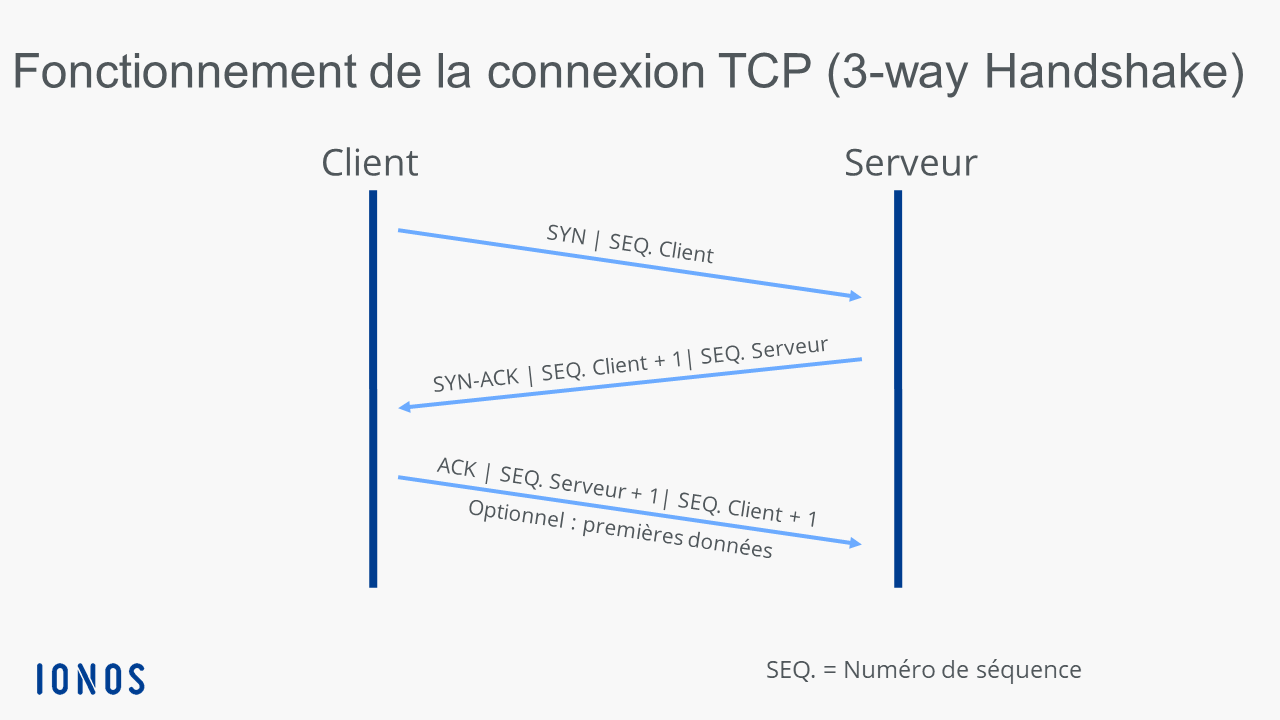
\includegraphics[width=10cm]{ressources/tcp-debut.png}
\captionof{figure}{Triple poignée de mains}
\label{echanges}
\end{figure}
\begin{activite}
\begin{enumerate}
\item Dans la fenêtre \emph{échanges de données}, vérifier le déroulement de la \emph{triple poignée de mains}.
\item Quel est le numéro de séquence de départ du client? Quel est celui du serveur?
\item Observer dans le détail des échanges (figure \ref{details}) l'incrémentation de ces deux numéros.
\item Quel est l'intérêt de cette succession d'échanges?
\item Dans le détail des échanges (figure \ref{details}) quelle est la ligne où le serveur web envoie les données de la page web?
\end{enumerate}
\end{activite}
\begin{figure}[!h]
\centering
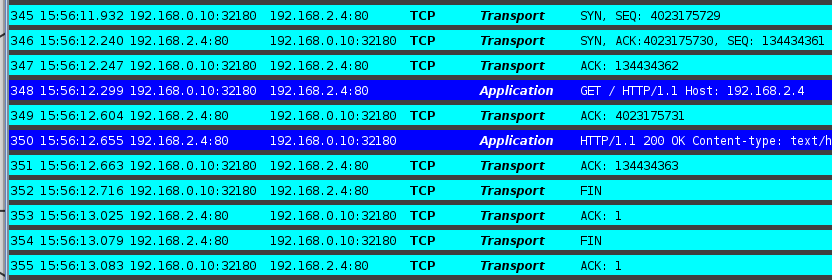
\includegraphics[width=14cm]{ressources/echanges-details.png}
\captionof{figure}{Détails des échanges}
\label{details}
\end{figure}


\end{Form}
\end{document}